\documentclass[10pt,a4paper]{report} 
% Style
\usepackage{amsfonts}
\usepackage{amsmath}
\usepackage{amssymb}
\usepackage[utf8]{inputenc}
\usepackage[T1]{fontenc}
\usepackage[english]{babel}
\usepackage{lmodern} 
\usepackage{graphicx}
\usepackage{color}
\usepackage{float}
\usepackage{url}


% Formler
\newcommand{\gaspedal}{\beta_{ped}}
\newcommand{\throttlewinkel}{\alpha_{th}}
\newcommand{\throttlewinkelacc}{\dot{\alpha}_{th}}
\newcommand{\throttledelay}{\tau_{th}}
\newcommand{\AFs}{\lambda}
\newcommand{\massenstrom}{\dot{m}}
\newcommand{\luftmassenstromat}{\dot{m}_{at}}
\newcommand{\luftmassenstromac}{\dot{m}_{ac}}
\newcommand{\etalvol}{\eta_{vol}}
\newcommand{\zylindergesamtvolumen}{V_D}
\newcommand{\throttletemp}{T_{bef,th}}
\newcommand{\injektierterbrennstoffmassenstrom}{\dot{m}_{fi}}
\newcommand{\brennstoffmasse}{m_f}
\newcommand{\brennstoffmassenstrom}{\dot{m}_{fc}}
\newcommand{\effektiveflache}{A_{eff}}
\newcommand{\etatildeign}{{\tilde \eta}_{ig} ( \lambda_{c}, \theta_{ign}, r_{c}, N_{e}, V_{d} )}


% Sources

% ---Title page ---



% ---Dokumen start---
\begin{document}



% ---Title page ---
\title{Localisation using microphone network\\Sensor fusion -- TSRT14}
\author{Group 12}
\maketitle

\abstract{This is a report for on of the laboration assignments in the course Sensor fusion (TSRT14) at LiTH.
  It consists of estimation and tracking och location for a robot that is moving in a audio sensor network.
Several different algorithms are used and compared to each other.}

% ---Innehållsförteckning---
\tableofcontents

\newpage
\chapter{Data gathering}
\label{Data gathering}
The data that is used in this report was gathered during a session at Laboteket.
The setup was a robot that followed a path around a track that was about one meter in diameter.
As the robot went around the track it emitted a pulse two times per second.
The sensor that were used was 7 microphones that could be placed anywhere around the track.
Three datasets were collected.
First a calibration set. This was collected by placing all the microphones on the same distant from the robot.
This was achived by placing all the microphones on a small segement of a circle with the robot in the center.
The robot was then setup to just emit the pulses and stay still.

After this was done the robot was set up to drive around the track while the microphones recorded data.
Two different setup were used. The placement of the microphones can be seen in Figure \ref{good_setup} and \ref{bad_setup}.
The first setup up was choosen to have microphones spread as even as possible around the track.
This will make the arrival times at the microphones as different as possible.
In the second setup the microphones are closer together and there should be less difference between the arrival time of different microphones.

The robot went around the track about two times for each recording session.
The recorded sound was then processed to find the arrival times for each pulse on every microphone.
These arrival times are then used for tracking and localisation.

The processing of the recordings are done by correlating the recorded signal with the pulse that was transmitted from the robot.
This will give large peaks where the pulses were recorded.

\begin{figure}[!h]
  \label{good_setup}
  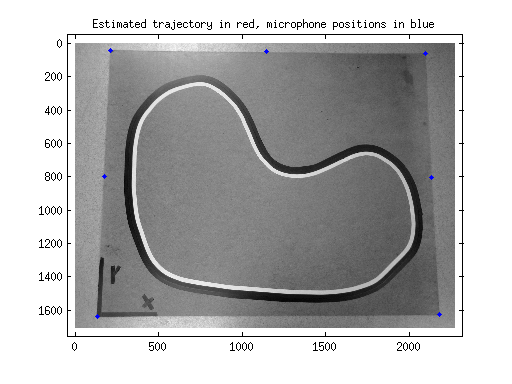
\includegraphics[scale=0.9]{microphone_pos_good.png}
  \caption{Microphone setup one.}
\end{figure}

\begin{figure}[!h]
  \label{bad_setup}
  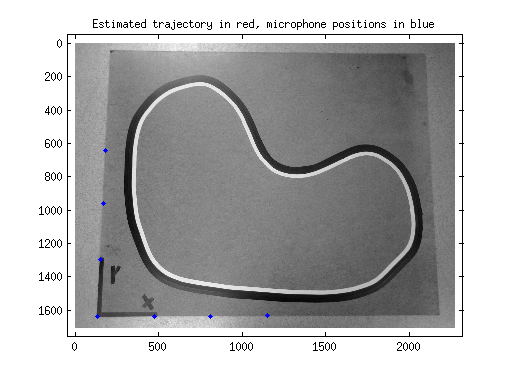
\includegraphics[scale=0.9]{microphone_pos_bad.png}
  \caption{Microphone setup two.}
\end{figure}

\newpage
\chapter{Tasks}
\label{Tasks}
The laboration assignment consisted of several task that needed to be completed. This is a description of how they were completed.

\newpage
\section{Calibration}
\label{Calibration}

\newpage
\section{Sensor modeling}
\label{Sensor modeling}
To do localisation and tracking, a model must be used to process the data in the datasets.
The algorithms used in this laboration need a function that maps the state of the robot to the measurments that has been recorded.
An important observation is that the time when the pulse was emitted from the robot is not known.
This means that either this time has to be estimated as a stat of the robot or that it is eliminated by using the differences of the arrival times in the microphones.
This gives two different sensor models.
In the sensormod toolbox that is used in the course these are reffered to as \emph{TDOA1} and \emph{TDOA2} respectively.
The TDOA1 model can be described using a three dimensional state variabel $x = [p^T, r_0]^T$ 
for the robot and the arrival times of the pulse as a 7-dimensional measurment $y$.
$p = [x1 x2]^T$ is the position of the robot. $r_0$ is the time that the pulse was transmitted from the robot.
The positions of the microphones are denoted $th^i$ where $i$ is the number of the microphone.
The model then becomes
\[
  \bar{y} = 
  \begin{bmatrix}
    |th^1 - p| + r_0 \\ 
    |th^2 - p| + r_0 \\ 
    |th^3 - p| + r_0 \\ 
    |th^4 - p| + r_0 \\ 
    |th^5 - p| + r_0 \\ 
    |th^6 - p| + r_0 \\ 
    |th^7 - p| + r_0 \\ 
  \end{bmatrix} + e
\]
$e$ is the measurment noise. This is estimated in the calibration stage of the asignment.
For simplicity this is assumed to be gaussian and independent.
This sensornetwork can be generated using the \emph{exsensor} funtion from the toolbox.
\begin{verbatim}
exsensor('tdoa1', 3, 1, 2);
\end{verbatim}

The model called TDOA2 uses a two dimensional state $x = p$ with the same $p$ as before.
The differences of the arrival times can then be used to eliminate $r_0$.
There are 7 different microphones wich mean that there are 21 different differences that can be constructed.
In the tasks we have used both a model with all these differences and 
a model with one microphone as a reference and only the differencies of the other microphones with respect to the reference microphone.
Using the difference means that the measurment $\bar{y}$ can't be used instead a new measurment $\tilde{y}$ is constructed by taking pairwise differencies of $\bar{y}$.
The measurment noise in this case can be estimated by taking the difference of the stochastic variables describing the independent measurment noise for each microphone.
For simplicity this new measurment noise is assumed to be independent with variance given by the sum of 
In the first case the model is

\[
  \tilde{y} = 
  \begin{bmatrix}
    |th^1 - p| - |th^2 - p| \\
    |th^1 - p| - |th^3 - p| \\
    |th^1 - p| - |th^4 - p| \\
    |th^1 - p| - |th^5 - p| \\
    |th^1 - p| - |th^6 - p| \\
    |th^1 - p| - |th^7 - p| \\
    |th^2 - p| - |th^3 - p| \\
    |th^2 - p| - |th^4 - p| \\
    |th^2 - p| - |th^5 - p| \\
    |th^2 - p| - |th^6 - p| \\
    |th^2 - p| - |th^7 - p| \\
    |th^3 - p| - |th^4 - p| \\
    |th^3 - p| - |th^5 - p| \\
    |th^3 - p| - |th^6 - p| \\
    |th^3 - p| - |th^7 - p| \\
    |th^4 - p| - |th^5 - p| \\
    |th^4 - p| - |th^6 - p| \\
    |th^4 - p| - |th^7 - p| \\
    |th^5 - p| - |th^6 - p| \\
    |th^5 - p| - |th^7 - p| \\
    |th^6 - p| - |th^7 - p| \\
  \end{bmatrix} + e
\]
\\*
This can also be generated with \emph{exsensor}.
\begin{verbatim}
exsensor('tdoa2', 7, 1, 2);
\end{verbatim}
The model with microphone 1 as the reference will be
\[
  \tilde{y} = 
  \begin{bmatrix}
    |th^1 - p| - |th^2 - p| \\
    |th^1 - p| - |th^3 - p| \\
    |th^1 - p| - |th^4 - p| \\
    |th^1 - p| - |th^5 - p| \\
    |th^1 - p| - |th^6 - p| \\
    |th^1 - p| - |th^7 - p| \\
  \end{bmatrix} + e
\]
\\*
This is generated using the \emph{sensormod} constructor.
\begin{verbatim}
h = '[';
for i = 2:7,
  h = [h sprintf('sqrt((x(1,:)-th(1)).^2+(x(2,:)-th(2)).^2) - ...
  sqrt((x(1,:)-th(%d)).^2+(x(2,:)-th(%d)).^2);', i*2-1, i*2)];
end
h = [h ']'];
sm = sensormod(h, [2 0 6 14])
\end{verbatim}
\newpage
\section{Configuration analysis}
\label{Configuration analysis}


\newpage
\section{Localisation}
\label{Localisationg}

\newpage
\section{Tracking}
\label{Tracking}

\newpage
\section{Sensitivity analysis}
\label{Sensitivity analysis}

\end{document}



%%% Local Variables: 
%%% TeX-PDF-mode: t 
%%% TeX-master: "rapport"
%%% End: 

